\documentclass[11pt,a4paper]{article}

\usepackage[margin=1in]{geometry}
\usepackage{amsmath,amssymb}
\usepackage{booktabs}
\usepackage{graphicx}
\usepackage{xcolor}
\usepackage{hyperref}
\usepackage{url}
\usepackage{natbib}
\usepackage{enumitem}
\usepackage{caption}
\usepackage{multirow}
\usepackage{array}
\usepackage{tabularx}
\usepackage{float}
\usepackage{microtype}

\hypersetup{
  colorlinks=true,
  linkcolor=blue!50!black,
  citecolor=blue!50!black,
  urlcolor=blue!40!black
}

\newcommand{\todo}[1]{\textcolor{gray}{\textit{#1}}}
\newcommand{\tbd}{\todo{TBD}}
\newcommand{\CTC}{\mathrm{CTC}}

\title{Measuring the Multilingual Token Tax:\\
Frontier Premiums and a Language-Conditional SuperBPE Bake-Off}

\author{
Aryan Jaden Verma\\
Frank Gonzalez
}

\date{}

\begin{document}
\maketitle

\begin{abstract}
Production language-model tokenizers remain English-centric: the same parallel content can require substantially more tokens in under-served scripts, inflating latency and---because commercial APIs bill per token---inference spend~\citep{petrov2023unfairness,ahia2023cost}.
We report three complementary studies.
First, we publish an empirical \emph{token-tax} table on FLORES-200 for Amharic, Odia, and dialectal Arabic (Egyptian, Moroccan), with Swahili and Hausa as Latin-script African controls, across frontier BPE tokenizers and a published SuperBPE baseline.
On OpenAI \texttt{o200k}, Amharic and Odia require $5.78\times$ and $4.99\times$ as many tokens as English for the same sentences; Llama and GLM push Odia above $12\times$.
These measured premiums replace the literature's broad $3$--$12\times$ range with language- and tokenizer-specific numbers.
Second, we train matched BPE and SuperBPE tokenizers~\citep{liu2025superbpe} on an equal-byte six-language corpus (960\,MB) and evaluate English-relative token premium, fertility, and Zipf deviation on FLORES.
SuperBPE lowers fertility for every whitespace-delimited language in the set, yet \emph{raises} English-relative premium for Mandarin ($0.912\to 1.082$) and Hungarian ($1.084\to 1.160$)---failure modes consistent with prior BPB evidence that SuperBPE underperforms BPE on these languages~\citep{chowdhury-woolf-2026-benchmarking}, and that make any tokenizer recommendation language-conditional.
Third, we run a Phase~0 language-model pilot: matched \texttt{olmo2\_100M} models trained for $\sim$2B equal tokens per arm.
Raw bits/token favors BPE by $+0.84$ micro-average, but fertility-normalized approximate bits-per-byte (UTF-8 bytes/token on FLORES) collapses the gap to roughly $+0.025$ on non-CJK languages, with SuperBPE slightly better only on Haitian Creole.
A planned 1B-parameter UniMax bake-off with true UTF-8 bits-per-byte evaluation is specified; those tables are left empty pending training.
\end{abstract}

\section{Introduction}
\label{sec:intro}

Tokenization converts Unicode text into a finite vocabulary of subword (or superword) units.
Although the map is language-agnostic in principle, vocabularies and merge schedules of production systems are overwhelmingly tuned to English and other high-resource Latin-script languages~\citep{petrov2023unfairness,arnett2025inequities}.
The result is systematic over-segmentation of other languages: longer token sequences for the same meaning, shorter usable context windows, and---crucially for deployed systems---higher API bills, because vendors charge per token~\citep{ahia2023cost}.

Prior work has framed this disparity as a ``token tax'' or ``script tax,'' often summarizing the gap with wide ranges such as $3$--$12\times$ English~\citep{dixit2026scripttax,somide2026african,petrov2023unfairness}.
Such ranges are useful as existence proofs but are hard to use for planning: they mix tokenizers, language samples, and metrics.
We contribute a locked, reproducible measurement on FLORES-200~\citep{goyal2022flores,nllb2022} for a geographically diverse 12-language set, with a highlighted \emph{target-script} slice---Amharic (Ethiopic), Odia (Orya), Egyptian and Moroccan Arabic---and Latin-script African controls (Swahili, Hausa).

A second question is whether algorithm choice can close the tax.
SuperBPE~\citep{liu2025superbpe} extends BPE with a second stage that learns whitespace-bridging ``superwords,'' reporting large English-centric efficiency and quality gains.
We ask whether those gains transfer under a multilingual equal-byte training regime that includes languages where SuperBPE has already been shown to underperform on BPB---Mandarin and Hungarian~\citep{chowdhury-woolf-2026-benchmarking}.
We train matched BPE and SuperBPE arms on 960\,MB of FineWeb~/FineWeb-2 text~\citep{penedo2024fineweb,penedo2025fineweb2} and evaluate on FLORES.
We find that SuperBPE is not uniformly preferable: fertility improves for five of six languages, but English-relative token premium worsens for Mandarin and Hungarian, aligning with that prior extrinsic result.
Any recommendation must therefore be language-conditional.

Downstream language-model quality is the natural next measurement.
In \S\ref{sec:study-c} we report a Phase~0 \texttt{olmo2\_100M} pilot under equal-token training and specify a deferred 1B UniMax bake-off~\citep{chung2023unimax} whose bits-per-byte tables remain empty pending training.

\paragraph{Contributions.}
\begin{enumerate}[leftmargin=*,itemsep=2pt]
  \item Encode-only FLORES token-tax audit for Amharic, Odia, dialectal Arabic, plus Swahili/Hausa controls; full matrices in the appendix.
  \item Matched SuperBPE-versus-BPE bake-off on six languages at equal-byte scale, with Mandarin and Hungarian as SuperBPE premium failures.
  \item A Phase~0 100M LM pilot (bits/token and fertility-normalized approx.\ BPB) plus a deferred 1B UniMax BPB evaluation skeleton.
\end{enumerate}

\section{Related Work}
\label{sec:related}

\paragraph{Cross-lingual tokenizer unfairness.}
\citet{petrov2023unfairness} show that parallel text can differ by up to roughly $15\times$ in token length across languages under multilingual tokenizers, and argue for fairer vocabularies.
\citet{ahia2023cost} connect the same phenomenon to commercial API pricing.
Subsequent ``script tax'' and ``African language tax'' studies~\citep{dixit2026scripttax,somide2026african} report fertility and English-relative premiums on African and Indic scripts.
\citet{arnett2025inequities} operationalize \emph{token premiums} as corpus token-count ratios on FLORES; morphology-focused analyses~\citep{arnett2024morphology} motivate including agglutinative languages such as Hungarian.

\paragraph{Superword tokenization.}
\citet{liu2025superbpe} introduce SuperBPE: stage~1 learns ordinary subwords under whitespace pretokenization; stage~2 lifts that restriction to form superwords.
Published SuperBPE models improve English-centric compression and 8B downstream scores.
\citet{chowdhury-woolf-2026-benchmarking} provide the first extrinsic cross-language BPB comparison of BPE, SuperBPE, and MorphBPE on English, Mandarin, and Hungarian: SuperBPE matches BPE on English but underperforms by $0.01$--$0.06$ BPB on Hungarian and Mandarin, suggesting that cross-whitespace merging is counterproductive outside English.
Our Study~B tests whether encode-time premiums under equal-byte multilingual training reproduce that language-conditional pattern.

\paragraph{Multilingual pretraining mixtures.}
\citet{chung2023unimax} propose UniMax sampling with an epoch cap to balance languages without over-repeating scarce data.
Our Study~C 1B bake-off (\S\ref{sec:study-c}) adopts UniMax over FineWeb-2 pools with a 20B-token budget measured on the BPE arm~\citep{hoffmann2022chinchilla,muennighoff2023scaling,olmo2025}.

\section{Metrics}
\label{sec:metrics}

Let $\mathbf{s}_{1:N}^{(\ell)}$ be the $N$ parallel FLORES-200 \texttt{devtest} sentences in language $\ell$ ($N{=}1012$).
For a tokenizer $h$ we define corpus token count
\begin{equation}
  \CTC(\ell; h) \;=\; \sum_{i=1}^{N} \bigl|\, h\!\bigl(\mathbf{s}_{i}^{(\ell)}\bigr)\,\bigr|,
\end{equation}
excluding BOS/EOS where the tokenizer would insert them.
Following~\citet{arnett2025inequities}, the \textbf{token premium} relative to English is
\begin{equation}
  \mathrm{premium}(\ell; h) \;=\; \frac{\CTC(\ell; h)}{\CTC(\mathrm{eng}; h)}.
\end{equation}
By construction, $\mathrm{premium}(\mathrm{eng}; h) = 1$ for every $h$.
\textbf{Fertility} is tokens per whitespace word after Unicode NFKC~\citep{petrov2023unfairness}; for Mandarin we also report tokens per character and caution against interpreting tokens/word.
\textbf{Characters per token} uses non-whitespace code points over $\CTC$.

\paragraph{API cost scaling.}
Commercial language-model APIs bill by token~\citep{ahia2023cost}.
For a fixed parallel payload, relative inference token spend therefore scales linearly with premium:
if language $\ell$ has premium $p$, it incurs $p$ times as many billed tokens as English under the same tokenizer and pricing tier.
We report premiums rather than dollarizing a student cohort; the conversion to currency is a single multiplication by the vendor's per-token rate.

\section{Study A: Frontier Token Tax}
\label{sec:study-a}

\subsection{Setup}

\paragraph{Languages.}
We evaluate the locked 12-language FLORES-200 set used by our efficiency validation:
Swahili, Hausa, Amharic, Odia, Mandarin, Egyptian Arabic, Moroccan Arabic, Hungarian, Ukrainian, English, Ayacucho Quechua, and Guarani.
The \emph{target-script} highlight is Amharic (\texttt{amh\_Ethi}), Odia (\texttt{ory\_Orya}), Egyptian Arabic (\texttt{arz\_Arab}), and Moroccan Arabic (\texttt{ary\_Arab}), with Swahili (\texttt{swh\_Latn}) and Hausa (\texttt{hau\_Latn}) as Latin-script African controls.

\paragraph{Tokenizers.}
Frontier BPE: OpenAI \texttt{o200k\_base}~\citep{openai2024o200k}, Llama~3.1~\citep{meta2024llama31}, Qwen2.5~\citep{qwen2024qwen25}, GLM-5.2~\citep{glm2025}.
Published SuperBPE: UW OLMo2-8B SuperBPE (t180k)~\citep{uwsuperbpe2025,liu2025superbpe}.
Multilingual baseline: NLLB-200 Unigram~\citep{nllb2022}.
All metrics are encode-only; no language-model generation is required.

\paragraph{Decision rule (pre-registered).}
We treat a fairer-tokenizer research program as worth pursuing if either (A)~at least one non-English language has premium $\ge 2$ on $\ge 2$ frontier BPE tokenizers, or (B)~mean fertility for a non-Latin / complex-morphology language is $\ge 2\times$ English on the same tokenizer.
Both clauses pass: five languages hit clause~A (\texttt{amh\_Ethi}, \texttt{ory\_Orya}, \texttt{quy\_Latn}, \texttt{grn\_Latn}, \texttt{hun\_Latn}).

\subsection{Results}

\begin{table}[t]
\centering
\caption{English-relative token premium on FLORES-200 \texttt{devtest} for target scripts and African Latin-script controls. Values are $\CTC_{\ell}/\CTC_{\mathrm{eng}}$. Full 12-language matrix in Table~\ref{tab:premium-full}.}
\label{tab:tax-highlight}
\small
\begin{tabular}{@{}lrrrrr@{}}
\toprule
Language & o200k & Llama & Qwen & GLM & SuperBPE \\
\midrule
English            & 1.00 & 1.00 & 1.00 & 1.00 & 1.00 \\
Swahili (control)  & 1.49 & 1.93 & 1.94 & 1.93 & 2.43 \\
Hausa (control)    & 1.55 & 1.97 & 1.94 & 1.94 & 2.47 \\
Egyptian Arabic    & 1.41 & 1.65 & 1.63 & 1.75 & 3.22 \\
Moroccan Arabic    & 1.48 & 1.71 & 1.69 & 1.81 & 3.26 \\
Amharic            & \textbf{5.78} & 7.59 & 4.05 & 7.59 & 5.90 \\
Odia               & \textbf{4.99} & \textbf{12.16} & 9.70 & \textbf{12.36} & 13.53 \\
\bottomrule
\end{tabular}
\end{table}

Table~\ref{tab:tax-highlight} replaces the literature's undifferentiated $3$--$12\times$ band with measured numbers.
On \texttt{o200k}, Amharic ($5.78\times$) and Odia ($4.99\times$) sit in the middle-to-upper part of that band; Llama and GLM push Odia above $12\times$, matching the upper end of prior summaries.
Dialectal Arabic is milder ($1.4$--$1.8\times$ on frontier BPE) but still a clear tax relative to English; the published SuperBPE baseline nearly doubles those Arabic premiums ($3.2\times$).
Swahili and Hausa---Latin script, African---land near $1.5\times$ on \texttt{o200k} and just under $2\times$ on Llama/Qwen/GLM, confirming that script family alone does not explain the Amharic/Odia gap.

\begin{figure}[t]
\centering
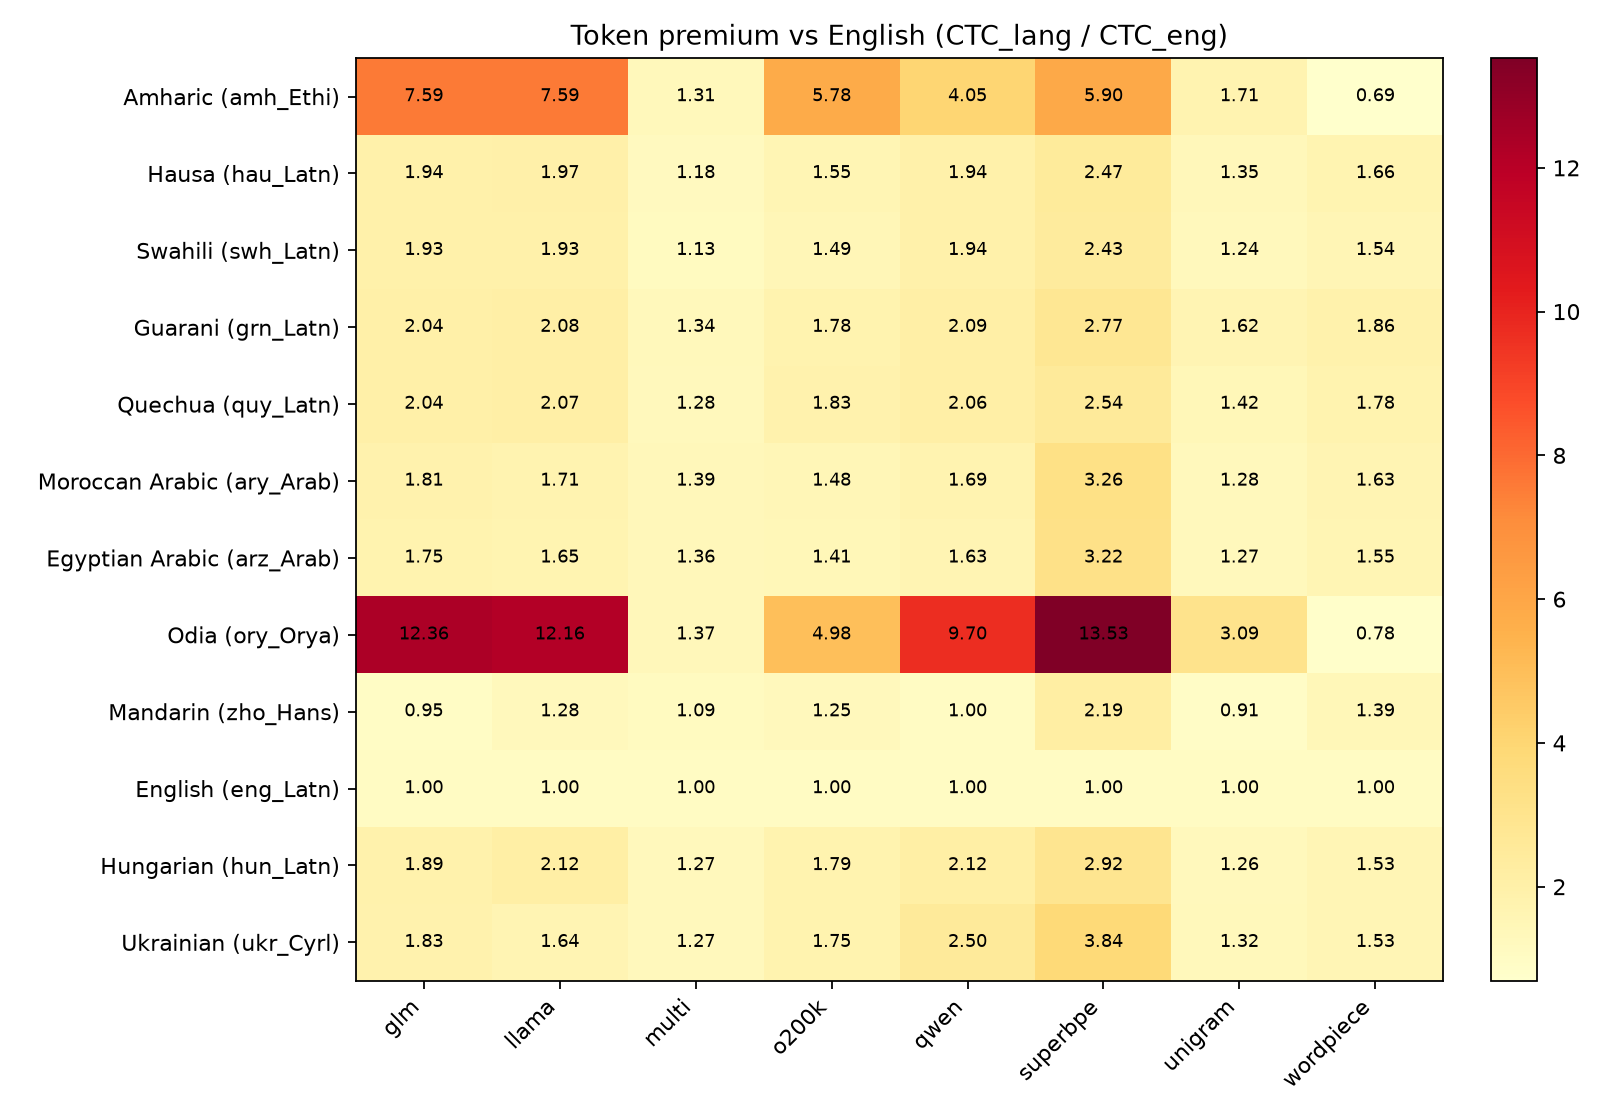
\includegraphics[width=\linewidth]{figures/efficiency_token_premium_heatmap.png}
\caption{Token-premium heatmap over the full 12-language efficiency set (Study~A). English is exactly $1.0$ by construction.}
\label{fig:heatmap}
\end{figure}

\begin{table}[t]
\centering
\caption{Continent mean token premium (non-English languages only).}
\label{tab:continent}
\small
\begin{tabular}{@{}lrrrr@{}}
\toprule
Continent & o200k & Llama & Qwen & SuperBPE \\
\midrule
Africa    & 2.94 & 3.83 & 2.64 & 3.60 \\
Americas  & 1.80 & 2.08 & 2.07 & 2.66 \\
Asia      & 2.28 & 4.20 & 3.51 & 5.55 \\
Europe    & 1.77 & 1.88 & 2.31 & 3.38 \\
\bottomrule
\end{tabular}
\end{table}

Continent means (Table~\ref{tab:continent}, Figure~\ref{fig:heatmap}) show Africa and Asia carrying the heaviest mean tax under frontier BPEs; Asia's SuperBPE mean ($5.55$) is dominated by Odia.
Because API cost scales with tokens, an Amharic request that is content-parallel to an English request costs $5.78\times$ as many \texttt{o200k} tokens---and therefore $5.78\times$ the token-metered spend---under the same pricing tier.

\section{Study B: SuperBPE versus BPE}
\label{sec:study-b}

\subsection{Setup}

\paragraph{Languages (separate scope).}
Study~B uses a different locked six-language set chosen for FineWeb-2 availability and typological coverage:
English, Hungarian, Mandarin, Hindi, Swahili, and Haitian Creole
(\texttt{eng\_Latn}, \texttt{hun\_Latn}, \texttt{zho\_Hans}, \texttt{hin\_Deva}, \texttt{swh\_Latn}, \texttt{hat\_Latn}).
This set is \emph{not} interchangeable with Study~A's twelve languages; Amharic, Odia, Hausa, and dialectal Arabic are absent from the bake-off.

\paragraph{Training.}
We train matched BPE and SuperBPE tokenizers with Gigatoken~\citep{roed2026gigatoken} via our SuperBPE-capable fork \texttt{supergigatoken}~\citep{verma2026supergigatoken} on an equal-byte \emph{scale} corpus: $160$\,MB per language, $960$\,MB total, drawn from FineWeb (English) and FineWeb-2 (other languages).
Equal bytes prevent a measured Creole or Swahili penalty from being a corpus-size artifact.
Vocabulary size is $100{,}000$; SuperBPE transitions at $80{,}000$.
Pair verification confirms that SuperBPE carries the BPE merge prefix through the transition point.
We pin \texttt{supergigatoken} at commit \texttt{00e61db} (branch \texttt{superbpe-stage1-pretokenizer}).
Each arm is encoded with the pre-tokenizer recorded in its own \texttt{tokenizer.json}.

\paragraph{Evaluation.}
FLORES-200 \texttt{devtest}: English-relative token premium, fertility (tokens/word), and Zipf--Mandelbrot Kolmogorov--Smirnov deviation $\mathrm{ks\_zipf}$~\citep{clauset2009power} under a matched-sentence, token-unit regime.
Lower $\mathrm{ks\_zipf}$ is closer to a pure Zipf distribution.
LM bits-per-byte is deferred to Study~C (\S\ref{sec:study-c}).

\subsection{Tokenizer-level results}

\begin{table}[t]
\centering
\caption{Study~B: English-relative token premium after equal-byte training. SuperBPE \emph{worsens} premium for Hungarian and Mandarin (bold).}
\label{tab:plan-a-premium}
\small
\begin{tabular}{@{}lrrc@{}}
\toprule
Language & BPE & SuperBPE & $\Delta$ \\
\midrule
English           & 1.000 & 1.000 & --- \\
Hungarian         & 1.084 & \textbf{1.160} & $+0.076$ \\
Mandarin          & 0.912 & \textbf{1.082} & $+0.170$ \\
Hindi             & 1.259 & 1.256 & $-0.003$ \\
Swahili           & 1.032 & 1.056 & $+0.024$ \\
Haitian Creole    & 1.034 & 1.004 & $-0.030$ \\
\bottomrule
\end{tabular}
\end{table}

\begin{table}[t]
\centering
\caption{Study~B: fertility (tokens / whitespace word). Mandarin is reported but not interpreted as tokens/word.}
\label{tab:plan-a-fertility}
\small
\begin{tabular}{@{}lrr@{}}
\toprule
Language & BPE & SuperBPE \\
\midrule
English        & 1.321 & 1.124 \\
Hungarian      & 1.676 & 1.526 \\
Mandarin       & 12.759 & 12.874 \\
Hindi          & 1.420 & 1.206 \\
Swahili        & 1.402 & 1.221 \\
Haitian Creole & 1.293 & 1.068 \\
\bottomrule
\end{tabular}
\end{table}

\begin{table}[t]
\centering
\caption{Study~B: Zipf deviation $\mathrm{ks\_zipf}$ (lower $=$ closer to Zipf). BPE is closer for all six languages.}
\label{tab:plan-a-zipf}
\small
\begin{tabular}{@{}lrr@{}}
\toprule
Language & BPE & SuperBPE \\
\midrule
English        & 0.121 & 0.297 \\
Hungarian      & 0.200 & 0.325 \\
Mandarin       & 0.292 & 0.310 \\
Hindi          & 0.134 & 0.301 \\
Swahili        & 0.163 & 0.304 \\
Haitian Creole & 0.080 & 0.294 \\
\bottomrule
\end{tabular}
\end{table}

\begin{figure}[t]
\centering
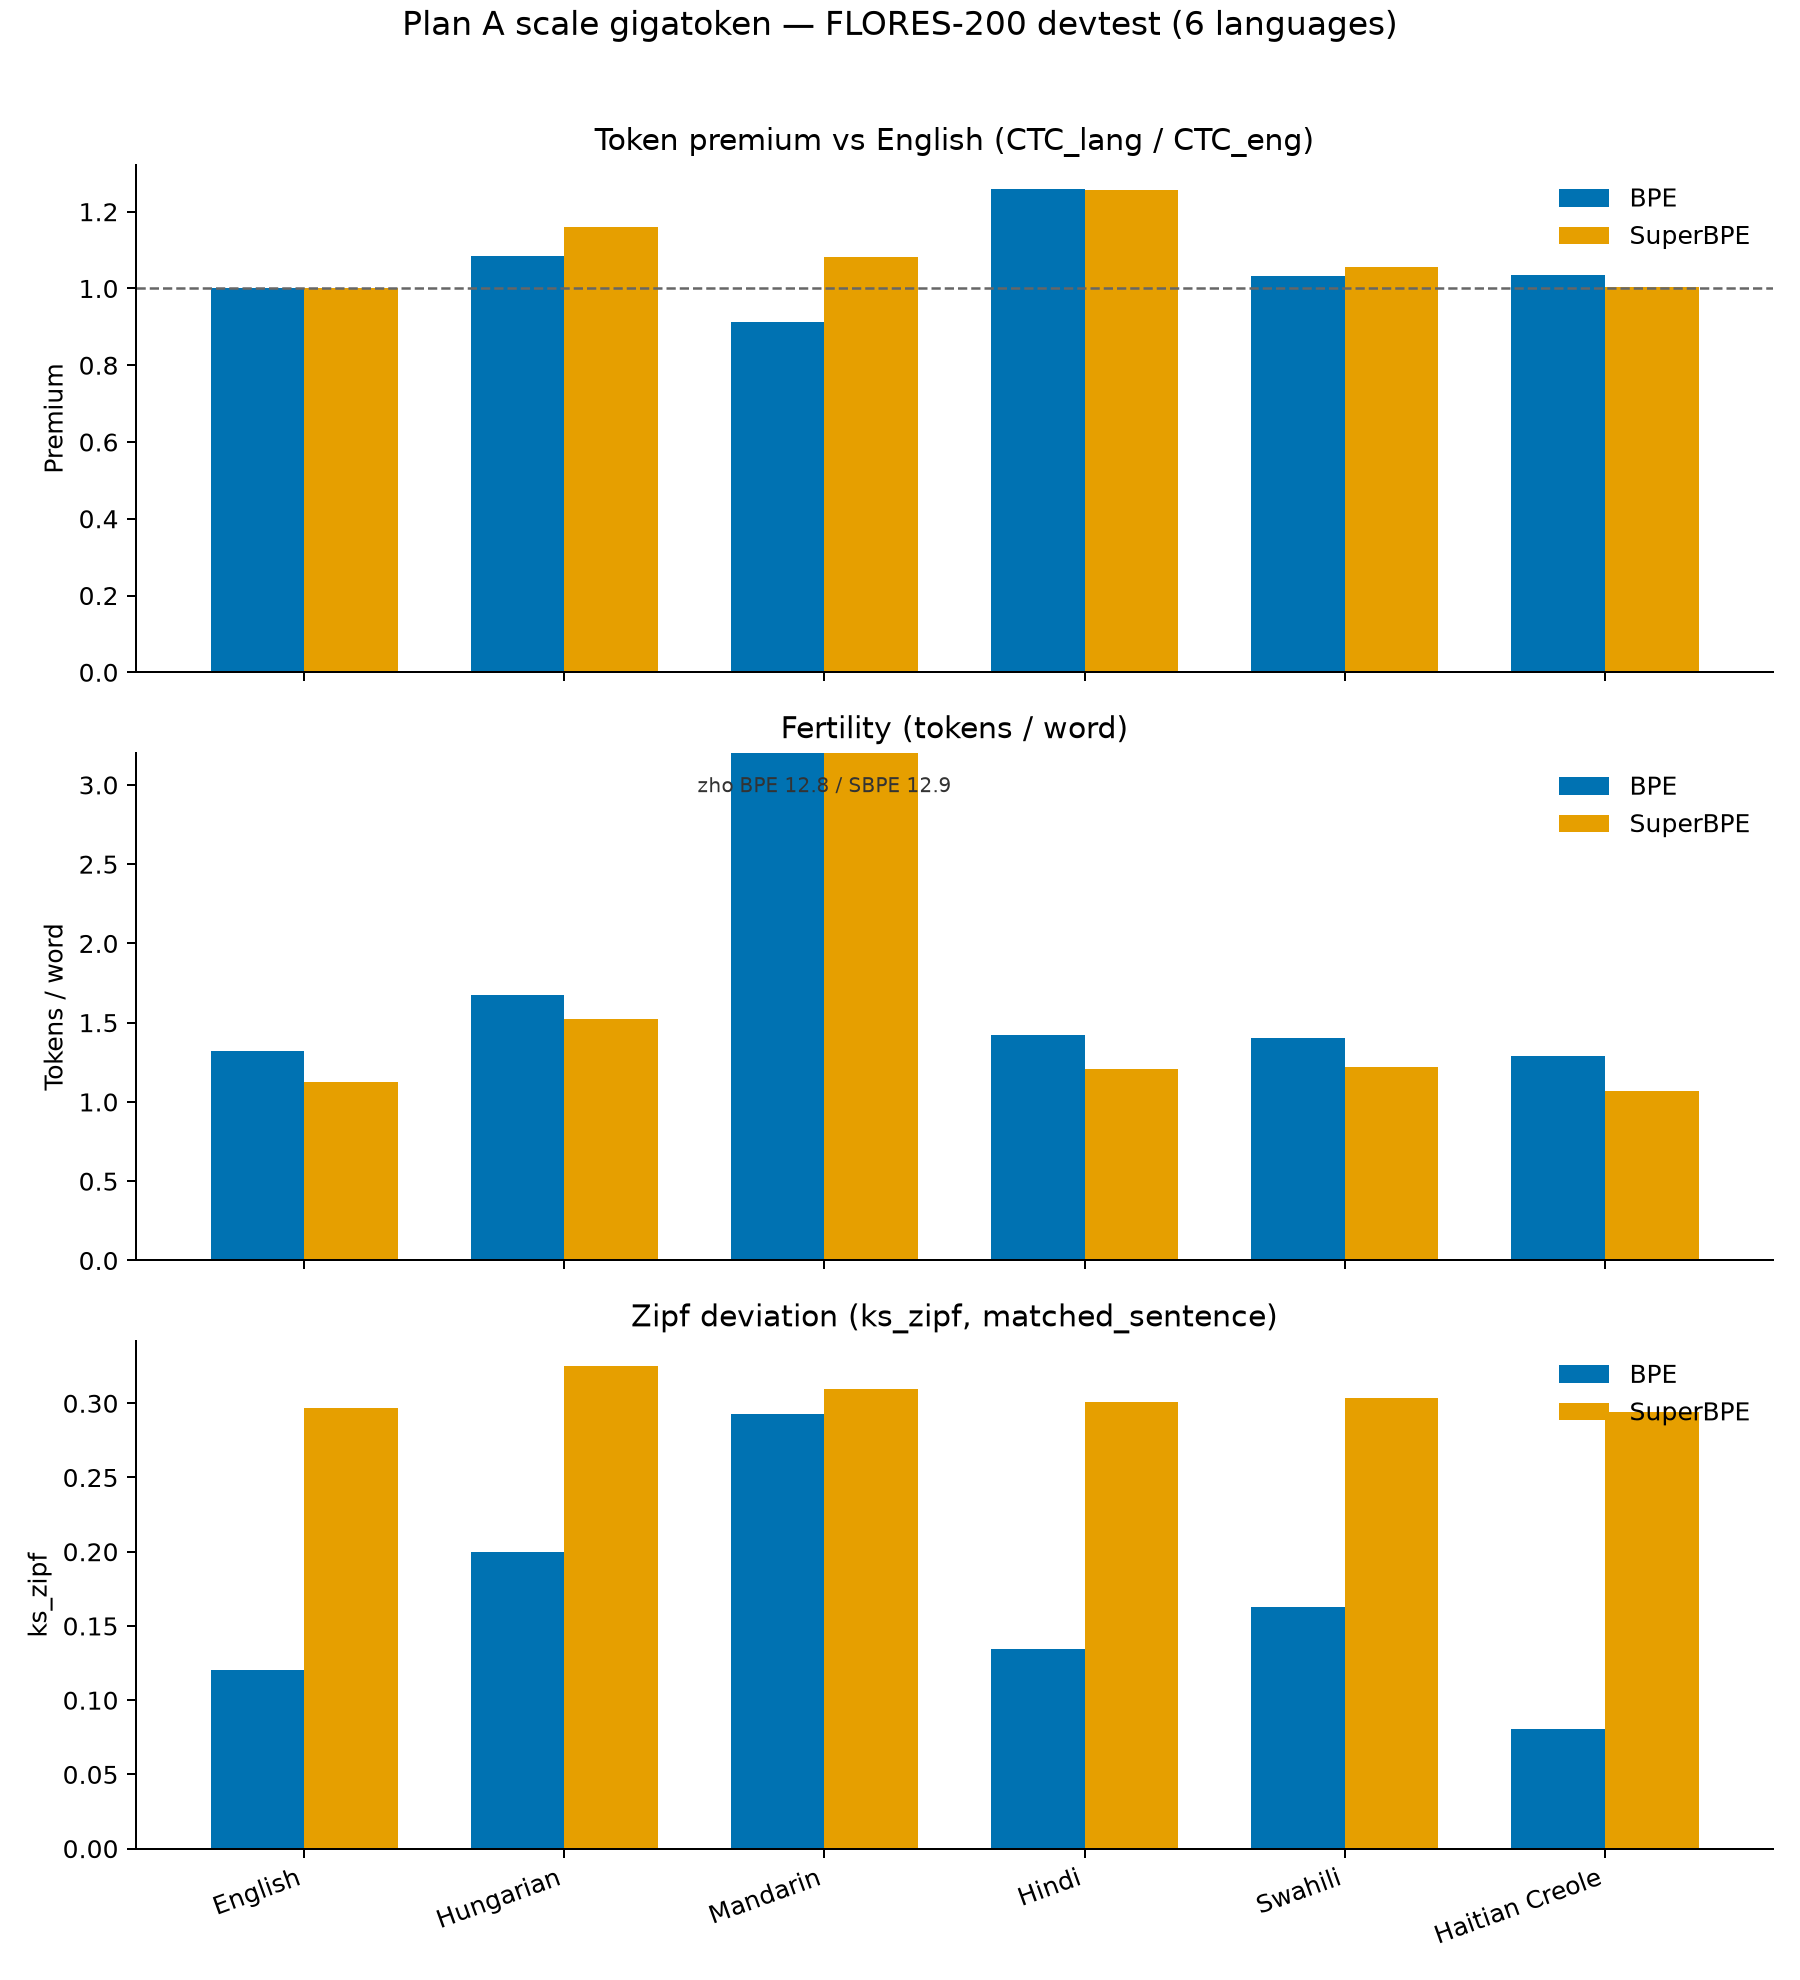
\includegraphics[width=\linewidth]{figures/plan_a_flores_suite_summary.png}
\caption{Study~B FLORES suite summary: token premium, fertility, and $\mathrm{ks\_zipf}$ for matched BPE and SuperBPE.}
\label{fig:plan-a-summary}
\end{figure}

Tables~\ref{tab:plan-a-premium}--\ref{tab:plan-a-zipf} and Figure~\ref{fig:plan-a-summary} show a mixed picture.
SuperBPE reduces fertility for every non-Mandarin language (Table~\ref{tab:plan-a-fertility}), consistent with superwords packing multi-word expressions.
Yet English-relative \emph{premium}---the quantity that tracks parallel API cost---moves the wrong way for Hungarian and Mandarin (Table~\ref{tab:plan-a-premium}), the same pair where \citet{chowdhury-woolf-2026-benchmarking} found SuperBPE worse than BPE by $0.01$--$0.06$ BPB.
Mandarin's BPE premium below $1.0$ ($0.912$) indicates that, under this equal-byte vocabulary, Mandarin is cheaper than English in tokens; SuperBPE erases that advantage ($1.082$).
Hungarian's premium rises from $1.084$ to $1.160$.
Haitian Creole is the clearest SuperBPE win on premium ($1.034\to 1.004$); Hindi is essentially tied.
On Zipf structure (Table~\ref{tab:plan-a-zipf}), BPE sits closer to a pure Zipf law for all six languages.

\paragraph{Language-conditional recommendation.}
Under equal-byte multilingual training and FLORES premium, we do \emph{not} recommend SuperBPE as a blanket upgrade.
Prefer SuperBPE where fertility and premium both improve (here: Haitian Creole; Hindi approximately neutral on premium with large fertility gain).
Prefer BPE where premium worsens---explicitly Mandarin and Hungarian in this suite---unless a downstream LM metric overturns the encode-only ranking.

\subsection{Trainer caveat (Hindi)}
\label{sec:hindi-caveat}

Our default trainer (\texttt{supergigatoken}~\citep{verma2026supergigatoken}, built on Gigatoken~\citep{roed2026gigatoken}) implements SuperBPE stage~2 without the official \texttt{STAGE2\_REGEX}, bounding units by separator, newline, and a maximum unit length of 128.
Relative to the official SuperBPE trainer~\citep{liu2025superbpe}, this yields a Hindi-specific compression advantage for the SuperBPE arm at small vocabularies (premium deltas of $-3.13\%$ at 4k and $-6.61\%$ at 16k in pilot cross-checks).
The BPE arm remains comparable across trainers.
Hindi SuperBPE premiums in Table~\ref{tab:plan-a-premium} should therefore be read as \emph{gigatoken-SuperBPE} numbers, not as a direct replication of published Liu et~al.\ SuperBPE.

\section{Study C: Language-Model Bake-Off}
\label{sec:study-c}
\label{sec:deferred}

Tokenizer-level metrics do not settle whether SuperBPE's fertility gains translate into better language modeling under a fixed compute budget.
Prior monolingual BPB evidence already favors BPE over SuperBPE for Mandarin and Hungarian~\citep{chowdhury-woolf-2026-benchmarking}.
Study~C asks the same question under matched multilingual pretraining with the Study~B Gigatoken~/\,\texttt{supergigatoken} tokenizers~\citep{roed2026gigatoken,verma2026supergigatoken}.
We execute a cheap Phase~0 pilot first, then specify a Phase~1 $\sim$1B UniMax run whose result tables remain empty.

\subsection{Experiment process}

Both phases share the Study~B tokenizers (\texttt{tokenizer/gigatoken-bpe/v1} and \texttt{tokenizer/gigatoken-superbpe/v1}, vocabulary size $100{,}000$, SuperBPE transition at $80{,}000$) and the same six FineWeb~/FineWeb-2 languages.
Phase~0 materializes equal-\emph{token} packed shards, trains matched \texttt{olmo2\_100M} models, evaluates held-out cross-entropy as bits/token, then fertility-normalizes with Study~B FLORES characters-per-token.
Phase~1 (deferred) materializes UniMax equal-\emph{byte} shards, trains matched \texttt{olmo2\_1B} models to equal FLOPs, and will report true UTF-8 bits-per-byte.

\subsection{Phase 0: 100M equal-token pilot}
\label{sec:phase0}

\paragraph{Training specifications.}
\begin{itemize}[leftmargin=*,itemsep=2pt]
  \item \textbf{Model:} \texttt{olmo2\_100M} via OLMo-core~\citep{olmo2025}.
  \item \textbf{Corpora:} \texttt{pretrain/fineweb2-phase0-equal-\{bpe,superbpe\}-2b/v1} (promoted under the eduLLM dataset standard).
  \item \textbf{Matching:} equal tokens---$\approx 2.0$B train tokens total, $6\times 333{,}316{,}096$ per language---not equal bytes.
  \item \textbf{Optimization:} $7629$ steps, sequence length $2048$, global batch $262{,}144$ tokens ($7629\times 262{,}144 = 1{,}999{,}896{,}576$ tokens), warmup $200$ steps, checkpoint every $2000$ steps; final checkpoint \texttt{step7629}.
  \item \textbf{Compute:} $8\times$A10G (\texttt{gpu-8xa10g}), team \texttt{scratch}, W\&B project \texttt{plan-b-phase0}.
\end{itemize}

\paragraph{Evaluation specifications.}
Held-out \texttt{val} shards only (no train-shard leakage).
We load \texttt{step7629} with OLMo-core \texttt{LMEvaluator} under padded FSL; Phase~0 val shards contain no EOS, so instances are non-overlapping sequence-length windows over each shard (final chunk may be shorter and pad-masked).
Primary metric is bits/token $=\mathrm{CE}/\ln 2$.
Because SuperBPE tokens cover more text on average, we also report an approximate bits-per-byte
\begin{equation}
  \widetilde{\mathrm{BPB}}(\ell)
  \;=\;
  \frac{\text{bits/token}(\ell)}{\text{UTF-8 bytes/token}(\ell)},
\end{equation}
where bytes/token is measured by encoding FLORES-200 \texttt{devtest} with the same gigatoken tokenizers (total UTF-8 bytes over $\CTC$).
This is still an approximation of Phase~0 val BPB (FLORES domain, not the FineWeb val shards), but it uses the correct UTF-8 denominator.

\paragraph{Results.}
Table~\ref{tab:phase0-bits} shows raw bits/token.
Micro-average bits/token is $5.45$ (BPE) versus $6.29$ (SuperBPE), a gap of $+0.84$ favoring BPE; Mandarin is essentially tied ($-0.05$).
Table~\ref{tab:phase0-approx-bpb} shows that fertility normalization collapses most of that gap: non-CJK micro $\widetilde{\mathrm{BPB}}$ differs by only $\approx{+}0.025$, and SuperBPE is slightly better on Haitian Creole alone.
Equal-token matching itself biases against SuperBPE (fewer unique bytes seen for the same token budget), so Phase~0 is a smoke gate, not a kill gate for the equal-byte 1B comparison.

\begin{table}[t]
\centering
\caption{Phase~0 held-out val LM eval (\texttt{olmo2\_100M} @ \texttt{step7629}, equal-token $\sim$2B). Bits/token $=\mathrm{CE}/\ln 2$.}
\label{tab:phase0-bits}
\small
\begin{tabular}{@{}lrrrrrr@{}}
\toprule
Language & BPE bits & BPE PPL & SuperBPE bits & SuperBPE PPL & $\Delta$ bits \\
\midrule
English        & 5.568 & 47.43 & 6.716 & 105.10 & $+1.148$ \\
Haitian Creole & 5.913 & 60.26 & 7.105 & 137.66 & $+1.192$ \\
Hindi          & 4.270 & 19.29 & 5.270 &  38.59 & $+1.000$ \\
Hungarian      & 5.132 & 35.07 & 5.993 &  63.71 & $+0.861$ \\
Swahili        & 5.316 & 39.84 & 6.175 &  72.25 & $+0.859$ \\
Mandarin       & 6.521 & 91.85 & 6.476 &  88.99 & $-0.046$ \\
\midrule
Micro          & 5.453 & 43.82 & 6.289 &  78.20 & $+0.836$ \\
\bottomrule
\end{tabular}
\end{table}

\begin{table}[t]
\centering
\caption{Phase~0 approximate BPB: bits/token divided by FLORES-200 UTF-8 bytes/token
(same gigatoken tokenizers). Negative $\Delta$ favors SuperBPE.
Domain caveat: fertility is FLORES, not Phase~0 FineWeb val text.}
\label{tab:phase0-approx-bpb}
\small
\begin{tabular}{@{}lrrr@{}}
\toprule
Language & BPE $\widetilde{\mathrm{BPB}}$ & SuperBPE $\widetilde{\mathrm{BPB}}$ & $\Delta$ \\
\midrule
English        & 1.219 & 1.252 & $+0.032$ \\
Haitian Creole & 1.419 & 1.409 & $-0.010$ \\
Hindi          & 0.461 & 0.483 & $+0.022$ \\
Hungarian      & 1.055 & 1.121 & $+0.066$ \\
Swahili        & 1.147 & 1.161 & $+0.014$ \\
Mandarin       & 1.425 & 1.428 & $+0.003$ \\
\midrule
Micro (non-CJK)& 1.060 & 1.085 & $+0.025$ \\
\bottomrule
\end{tabular}
\end{table}

\subsection{Phase 1: 1B UniMax bake-off (deferred)}
\label{sec:phase1}

We plan a matched OLMo-class~\citep{olmo2025} $\sim$1B pretraining run for each arm under the protocol that actually matches the SuperBPE hypothesis:

\begin{itemize}[leftmargin=*,itemsep=2pt]
  \item \textbf{Model:} \texttt{olmo2\_1B}; sequence length $2048$; BPE arm $80{,}200$ steps ($\approx$21B tokens); SuperBPE continues from equal-bytes ($\approx$71{,}986 steps) to equal FLOPs at $80{,}200$.
  \item \textbf{Corpora:} \texttt{pretrain/fineweb2-unimax-\{bpe,superbpe\}-20b/v1}.
  \item \textbf{Matching:} same \emph{bytes} (not the same token count); SuperBPE then catches up to equal FLOPs.
  \item \textbf{Mixture:} UniMax~\citep{chung2023unimax} with a 4-epoch cap~\citep{muennighoff2023scaling}; Haitian Creole is the binding language ($\approx 3.96\%$), the other five $\approx 19.21\%$ each.
  \item \textbf{Compute plan:} \texttt{gpu-8xh100} ($\approx$\$1.8k both arms at equal FLOPs).
  \item \textbf{Eval:} true UTF-8 bits-per-byte on held-out val / FLORES (primary); AmericasNLP placeholder unchanged.
\end{itemize}

Tables~\ref{tab:bpb-flores} and~\ref{tab:bpb-americas} are placeholders to be filled after training.

\begin{table}[t]
\centering
\caption{Deferred: bits-per-byte on FLORES-200 after $\sim$1B OLMo pretraining (20B-token BPE budget). \todo{To be filled after Plan~B 1B training.}}
\label{tab:bpb-flores}
\small
\begin{tabular}{@{}lcc@{}}
\toprule
Language & BPE BPB & SuperBPE BPB \\
\midrule
English        & \tbd & \tbd \\
Hungarian      & \tbd & \tbd \\
Mandarin       & \tbd & \tbd \\
Hindi          & \tbd & \tbd \\
Swahili        & \tbd & \tbd \\
Haitian Creole & \tbd & \tbd \\
\midrule
Mean           & \tbd & \tbd \\
\bottomrule
\end{tabular}
\end{table}

\begin{table}[t]
\centering
\caption{Deferred: bits-per-byte on AmericasNLP evaluation sets. \todo{To be filled after Plan~B 1B training.}}
\label{tab:bpb-americas}
\small
\begin{tabular}{@{}lcc@{}}
\toprule
Language / set & BPE BPB & SuperBPE BPB \\
\midrule
\todo{(language)} & \tbd & \tbd \\
\todo{(language)} & \tbd & \tbd \\
\midrule
Mean              & \tbd & \tbd \\
\bottomrule
\end{tabular}
\end{table}

\section{Discussion}
\label{sec:discussion}

\paragraph{Replacing the $3$--$12\times$ range.}
Study~A shows that the familiar range is not wrong so much as underspecified.
On \texttt{o200k}, Amharic ($5.78\times$) and Odia ($4.99\times$) sit inside it; on Llama/GLM, Odia exceeds $12\times$.
Dialectal Arabic and the Swahili/Hausa controls show that African languages are not uniformly taxed: Latin-script Swahili/Hausa are near $1.5$--$2\times$, while Ethiopic Amharic is several times worse.
Reporting language $\times$ tokenizer cells is more actionable for API cost planning than a single interval.

\paragraph{Controls matter.}
Without Swahili and Hausa, one might attribute the Africa continent mean ($2.94$ on \texttt{o200k}) entirely to ``African languages.''
The control row shows that the Amharic outlier drives much of that mean; Latin-script African languages behave closer to other Latin mid-resource languages.

\paragraph{SuperBPE is language-conditional.}
Study~B's Mandarin and Hungarian failures on English-relative premium are the load-bearing result for tokenizer choice, and they corroborate the BPB ranking of~\citet{chowdhury-woolf-2026-benchmarking} on the same two languages.
Fertility alone would recommend SuperBPE for Hungarian; premium---the API-relevant parallel-length ratio---would not.

\paragraph{Phase~0 does not settle 1B.}
Raw bits/token in Table~\ref{tab:phase0-bits} would appear to kill SuperBPE; fertility-normalized Table~\ref{tab:phase0-approx-bpb} shows most of that gap was token length, not modeling quality, and the ranking remains language-conditional (Haitian Creole favors SuperBPE; Hungarian and Hindi favor BPE).
Phase~0 also used equal-\emph{token} matching, which starves SuperBPE of bytes relative to Plan~B's equal-byte protocol.
Until Tables~\ref{tab:bpb-flores}--\ref{tab:bpb-americas} are filled under equal bytes and true UTF-8 BPB, we treat encode-time premium as the conservative decision metric for cost-sensitive deployments, with Chowdhury and Woolf's extrinsic gap as prior evidence that LM quality is unlikely to reverse the Mandarin/Hungarian call.

\section{Limitations}
\label{sec:limitations}

Study~A is encode-only: it measures token tax, not downstream task quality.
Study~B's language set excludes Amharic, Odia, Hausa, and dialectal Arabic, so the SuperBPE recommendation does not yet cover Study~A's highest-tax scripts.
The three studies in this codebase (12-language efficiency, 18-language Zipf, 6-language Plan~A/B) use non-overlapping language locks; numbers must not be pooled without labels.
Gigatoken~/\,\texttt{supergigatoken}'s Hindi SuperBPE stage-2 deviation (\S\ref{sec:hindi-caveat}) means Hindi SuperBPE premiums are not directly comparable to published Liu et~al.\ numbers.
Phase~0 matches equal tokens rather than equal bytes, and its $\widetilde{\mathrm{BPB}}$ uses FLORES UTF-8 bytes/token rather than paired byte lengths on the Phase~0 FineWeb val shards (domain mismatch).
The 1B LM bake-off is specified but not executed; Tables~\ref{tab:bpb-flores}--\ref{tab:bpb-americas} are empty by design.

\section{Conclusion}
\label{sec:conclusion}

We measured a FLORES token-tax table for Amharic, Odia, and dialectal Arabic with Swahili/Hausa controls.
Tokenizer-specific premiums replace the literature's $3$--$12\times$ range: Amharic $5.78\times$ and Odia $4.99\times$ on \texttt{o200k}; Odia above $12\times$ on Llama and GLM.
Because APIs bill per token, these premiums are relative cost multipliers for parallel content.
A matched SuperBPE-versus-BPE bake-off at equal-byte scale shows SuperBPE improving fertility broadly but worsening English-relative premium for Mandarin and Hungarian, so tokenizer choice must be language-conditional.
A Phase~0 \texttt{olmo2\_100M} pilot shows that raw bits/token strongly favors BPE under equal-token training, but fertility-normalized approximate BPB largely closes the gap and remains language-conditional.
Filling the deferred 1B equal-byte BPB tables is the remaining step before a quality-aware recommendation.

\section*{Acknowledgments}
FLORES-200~\citep{goyal2022flores,nllb2022}, FineWeb~/FineWeb-2~\citep{penedo2024fineweb,penedo2025fineweb2}, SuperBPE~\citep{liu2025superbpe}, Gigatoken~\citep{roed2026gigatoken}, \texttt{supergigatoken}~\citep{verma2026supergigatoken}, and the OLMo stack~\citep{olmo2025} made these measurements possible.

\bibliographystyle{plainnat}
\bibliography{references}

\appendix
\section{Full Study~A Premium Matrix}
\label{app:full-premium}

\begin{table*}[t]
\centering
\caption{Full English-relative token premium matrix (Study~A, FLORES-200 \texttt{devtest}).}
\label{tab:premium-full}
\small
\begin{tabular}{@{}lrrrrr@{}}
\toprule
Language & o200k & Llama & Qwen & GLM & SuperBPE \\
\midrule
English (\texttt{eng\_Latn})           & 1.00 & 1.00 & 1.00 & 1.00 & 1.00 \\
Hungarian (\texttt{hun\_Latn})         & 1.79 & 2.12 & 2.12 & 1.89 & 2.92 \\
Mandarin (\texttt{zho\_Hans})          & 1.25 & 1.28 & 1.00 & 0.95 & 2.19 \\
Ukrainian (\texttt{ukr\_Cyrl})         & 1.75 & 1.64 & 2.50 & 1.83 & 3.84 \\
Swahili (\texttt{swh\_Latn})           & 1.49 & 1.93 & 1.94 & 1.93 & 2.43 \\
Hausa (\texttt{hau\_Latn})             & 1.55 & 1.97 & 1.94 & 1.94 & 2.47 \\
Amharic (\texttt{amh\_Ethi})           & 5.78 & 7.59 & 4.05 & 7.59 & 5.90 \\
Odia (\texttt{ory\_Orya})              & 4.99 & 12.16 & 9.70 & 12.36 & 13.53 \\
Egyptian Arabic (\texttt{arz\_Arab})   & 1.41 & 1.65 & 1.63 & 1.75 & 3.22 \\
Moroccan Arabic (\texttt{ary\_Arab})   & 1.48 & 1.71 & 1.69 & 1.81 & 3.26 \\
Quechua (\texttt{quy\_Latn})           & 1.83 & 2.07 & 2.06 & 2.04 & 2.54 \\
Guarani (\texttt{grn\_Latn})           & 1.78 & 2.08 & 2.09 & 2.04 & 2.77 \\
\bottomrule
\end{tabular}
\end{table*}

\section{Additional Study~B Panels}
\label{app:plan-a-panels}

\begin{figure}[h]
\centering
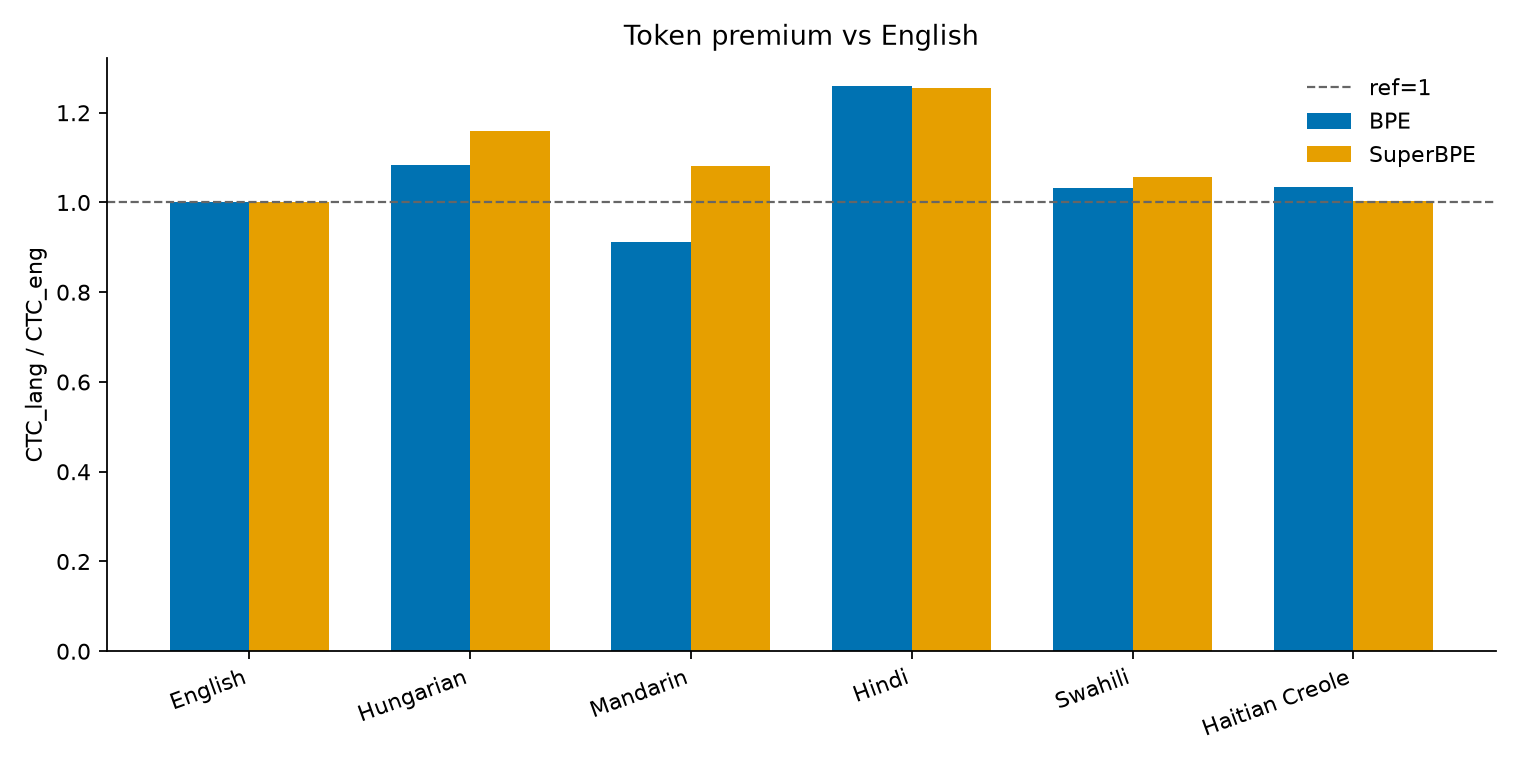
\includegraphics[width=0.95\linewidth]{figures/plan_a_token_premium.png}
\caption{Study~B token premium by language.}
\label{fig:plan-a-premium}
\end{figure}

\begin{figure}[h]
\centering
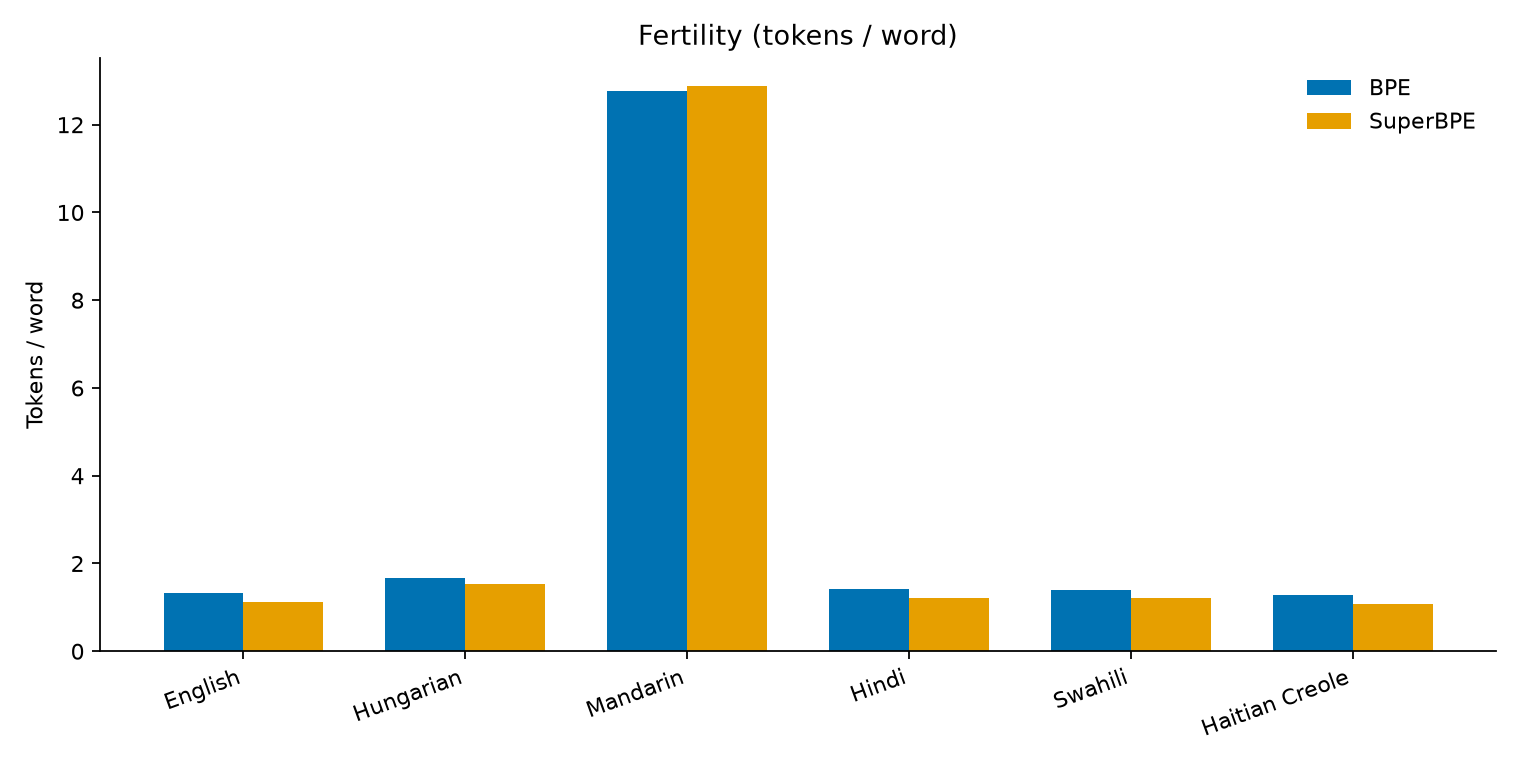
\includegraphics[width=0.95\linewidth]{figures/plan_a_fertility.png}
\caption{Study~B fertility by language.}
\label{fig:plan-a-fertility}
\end{figure}

\begin{figure}[h]
\centering
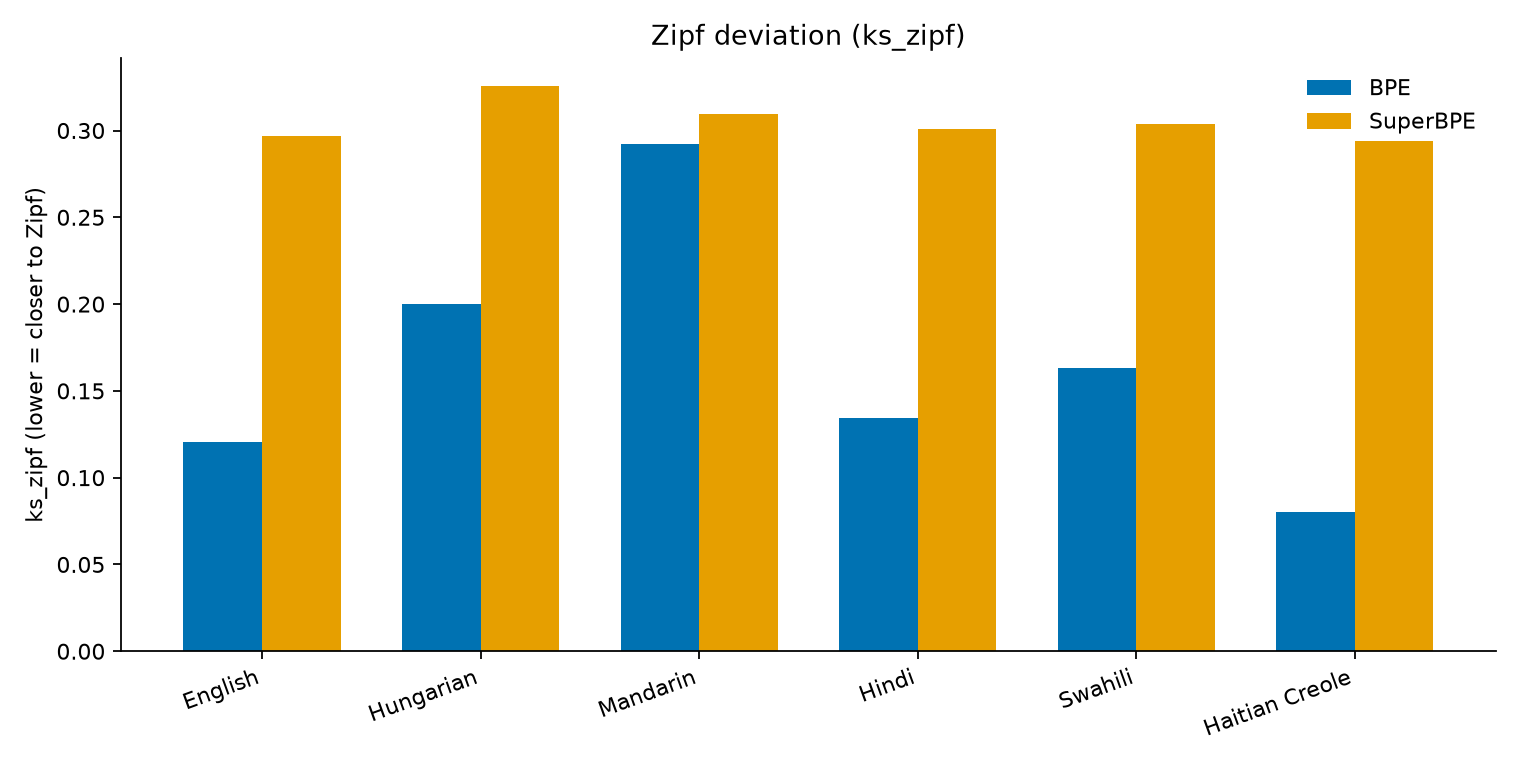
\includegraphics[width=0.95\linewidth]{figures/plan_a_ks_zipf.png}
\caption{Study~B $\mathrm{ks\_zipf}$ by language.}
\label{fig:plan-a-zipf}
\end{figure}

\end{document}
